\documentclass{stud-conf-pmk}

% Дополнительные пакеты для набора более сложных таблиц.
\usepackage{multirow}
\usepackage{diagbox}

\begin{document}
\year{2026}

\begin{paper}
\author[Иванов И.\,И.]{Иванов Иван Иванович}
\title{Название статьи}
\speciality{Прикладная математика и информатика}
\student{Студент магистратуры} % Студент/студентка магистратуры/бакалавриата.
\presented{Представил декан факультета ПМиК С.\,М.\,Дудаков}
%\presented{Представил заведующий кафедрой математической статистики и системного анализа В.\,Н.\,Михно}
%\presented{Представила доцент кафедры информатики В.\,Л.\,Волушкова}
\UDC{???, ???} % УДК через запятую.
\abstract{Аннотация содержит краткое описание полученных результатов.
Объем аннотации должен составлять 300--500 печатных знаков.}
\keywords{студенческая научная конференция, шаблон статьи, система \LaTeX}
\maketitle

\introduction

Введение содержит описание темы исследования с обоснованием актуальности.

\section{Набор текста}

\LaTeX{} автоматически расставляет пробелы в тексте и в формулах.
Важный \emph{термин} можно выделить разрядкой. В русских текстах
используются кавычки типа <<ёлочки>>. Букву <<ё>> нужно писать с точками: модель Эрдёша\,--\,Реньи, теорема Лёба. Многоточие пишется как
\dots, а не как ... Примеры использования диакритических знаков: \"{o},
\'{e}, \`{a}, \^{u}, \c{c}. Пустая строка в исходном файле завершает
абзац.

Дефис используется внутри одного слова (теорема Рыль"=Нардзевского,
контекстно-свободная грамматика). Короткое тире используется при описании
диапазонов (стр. 10--20). Длинное тире используется между словами
(дерево~--- это граф). Перед длинным тире поставлен неразрывный пробел,
чтобы тире и предыдущее слово не попали на разные строки.

\section{Формулы}

Включные формулы: $1+2=3$, $a+a+a=3a$. Формулы с индексами:
$x_1+x_2=x_2+x_1$, $a^2-b^2=(a-b)(a+b)$, $x_5^{20}<y_{17}^{1000}$.
Умножение в математических формулах записывается как $\cdot$ или $\times$,
а не $*$.

Греческие буквы: $\alpha$, $\beta$, $\gamma$, $\omega$, $\Gamma$,
$\Lambda$, $\Xi$, $\Upsilon$.

Выключные формулы:
$$(3x^2-2x+7)'=6x-2.$$

Диакритические знаки:
$$\bar x,\qquad \hat y,\qquad \vec{z},\qquad \tilde{u},\qquad
\dot{v},\qquad \ddot{w},\qquad \widehat{abc},\qquad \widetilde{xyz}.$$

Множества:
$$x \in A,\qquad y \notin B,\qquad A \subseteq B,\qquad
\overline{A \cap B}=\overline{A} \cup \overline{B}.$$

Обыкновенные дроби:
$$\frac{1}{2}+\frac{3}{4}=\frac{5}{4}.$$

Пределы:
$$\lim_{n \to \infty}\limits \frac{1}{n}=0.$$

Стандартные функции:
$$\sin \pi=0,\qquad \cos \frac{\pi}{4}=\frac{\sqrt{2}}{2},\qquad
\log_2 8=3,\qquad \max\{1,2\}=2.$$

Русский текст в формулах:
$$\tg x \textup{ не определено при } x=\frac{\pi}{2}\pm\pi n$$
или
$$\text{$\tg x$ не определено при $x=\frac{\pi}{2}\pm\pi n$}.$$

Неопределенный интеграл:
$$\int\sin x\,dx=-\cos x+C.$$

Определенный интеграл:
$$\int_a^b \limits F'(x)\,dx=F(b)-F(a).$$

Кратные интегралы:
$$\iiint\limits_V \left(\frac{\partial P}{\partial x}+
\frac{\partial Q}{\partial y}+\frac{\partial R}{\partial z}\right)\,dV=
\iint\limits_S P\,dy\,dz+Q\,dx\,dz+R\,dx\,dy.$$

%Суммы:
%$$\sum_{n=0}^\infty x^n=\frac{1}{1-x} \textup{ при } |x|<1.$$
%
%Произведения:
%$$n!=\prod_{k=1}^n k.$$
Суммы и произведения:
$$\sum_{n=0}^\infty x^n=\frac{1}{1-x} \textup{ при } |x|<1,\qquad
n!=\prod_{k=1}^n k.$$

Логические формулы:
$$(\lnot x \lor y) \to (x \oplus z),\qquad
(\forall x)(\exists y)(x<y \land P(y)).$$
%$$(\forall x)(\exists y)((P(x) \land Q(x,y)) \to \lnot (R(x) \lor P(y))).$$

Большие скобки:
$$\left(1+\frac{1}{2}\right)^2=\frac{9}{4}.$$

Разбор случаев:
$$\sign(x)=\begin{cases}
1, & \textup{если } x>0\\
0, & \textup{если } x=0\\
-1, & \textup{если } x<0\\
\end{cases}$$

Нумерация формул:
\begin{equation}
\label{eq1}
a^2-b^2=(a-b)(a+b).
\end{equation}
Из формулы~\eqref{eq1} следует, что
$$5^2-2^2=(5-2)(5+2)=3 \cdot 7=21,$$
поэтому окончательно получаем
$$5^2-2^2=21.$$

Несколько формул подряд:
\begin{gather}
x+y=y+x,\label{eq2}\\
(x+y)+z=x+(y+z).\label{eq3}
\end{gather}
Подставляя~\eqref{eq2} в~\eqref{eq3}, получаем
$$(y+x)+z=x+(y+z).$$

Несколько формул подряд без номеров:
\begin{gather*}
x+y=y+x,\\
(x+y)+z=x+(y+z).
\end{gather*}

Выравнивание формул:
\begin{align*}
1+2+3&=6&1 \cdot 2 \cdot 3&=6\\
1+2+3+4&=3+7&1 \cdot 2 \cdot 3 \cdot 4&=2 \cdot 12
\end{align*}

Другое выравнивание формул:
\begin{alignat*}{3}
x&{}+{}&2y&{}-{}&7z&=0\\
10x&{}-{}&y&{}+{}&18z&=9\\
2x&{}+{}&4y&{}+{}&6z&=-1
\end{alignat*}

Система уравнений:
$$\left\{
\begin{aligned}
x+y&=3\\
x^2+y^2&=7
\end{aligned}
\right.$$

Другая система уравнений:
$$\left\{\begin{alignedat}{3}
x&{}+{}&2y&{}-{}&7z&=0\\
10x&{}-{}&y&{}+{}&18z&=9\\
2x&{}+{}&4y&{}+{}&6z&=-1
\end{alignedat}\right.$$

Перенос длинных формул:
\begin{multline*}
1+2+3+4+5+6+7+8+9+10=\\
=10+9+8+7+6+5+4+3+2+1.
\end{multline*}

Несколько переносов в одной формуле:
\begin{multline*}
1+2+3+4+5+6+7+8+9+10=\\
=1+2+3+4+5+10+9+8+7+6=\\
=10+9+8+7+6+5+4+3+2+1.
\end{multline*}

\section{Списки}

Маркированный список. На этапе нормализации данных мы можем провести
следующие операции.
\begin{itemize}
\item Удаление пунктуации и специальных символов.
\item Приведение текста к нижнему регистру.
\item Удаление стоп-слов.
\end{itemize}
Перечислим некоторые из наиболее популярных моделей машинного обучения:
\begin{itemize}
\item наивный байесовский классификатор;
\item метод опорных векторов;
\item логистическая регрессия.
\end{itemize}

Нумерованный список. Были выполнены следующие задачи.
\begin{enumerate}
\item Проведен обзор и изучены теоретические основы существующих моделей и
методов прогнозирования временных рядов.
\item Разработана программная реализация гибридного метода анализа
временных рядов на основе алгоритмов ARIMA и XGBoost на языке
программирования R.
\item Проведен анализ результатов работы написанной программы.
\end{enumerate}


\section{Таблицы и рисунки}

В табл.~\ref{table1} и~\ref{table2} приведены примеры простых таблиц.
Табл.~\ref{table3} содержит объединенные ячейки. Для набора
табл.~\ref{table4} необходимо подключить пакет \verb|multirow|, а для
табл.~\ref{table5}~--- пакет \verb|diagbox|. В табл.~\ref{table6}
приведена таблица истинности конъюнкции.

\begin{table}
\centering
\caption{Точность моделей.}
\begin{tabular}{|l|l|l|l|}
\hline
& NBC & KNN & SVM\\
\hline
Новости & 92\% & 90\% & 94\%\\
\hline
Книги & 73\% & 67\% & 78\%\\
\hline
\end{tabular}
\label{table1}
\end{table}

\begin{table}
\centering
\caption{Время обучения.}
\begin{tabular}{|*{8}{l|}}
\hline
& NBC & KNN & SVM & LR & RF & RNN & CNN\\
\hline
Новости & 2{,}5 с & 3{,}5 с & 3 с & 4 с & 36 с & 27 с & 27 с \\
\hline
Книги & 50 с & 52 с & 53 с & 54 с & 150 с & 35 с & 35 с \\
\hline
\end{tabular}
\label{table2}
\end{table}

\begin{table}
\centering
\caption{Значения критерия Спирмена.}
\begin{tabular}{|c|c|c|c|c|c|c|}
\cline{2-7}
\multicolumn{1}{c|}{} & \multicolumn{2}{c|}{2-граммы} & \multicolumn{2}{c|}{3-граммы} & \multicolumn{2}{c|}{4-граммы}\\
\hline
Автор & $J_{p}$ & $z^{*}$ & $J_{p}$ & $z^{*}$ & $J_{p}$ &
$z^{*}$\\
\hline
A & 58,288 & 28,687 & 33,645 & 28,316 & 15,592 & 14,271\\
\hline
B & 54,897 & 28,344 & 32,115 & 27,447 & 14,031 & 13,065\\
\hline
C & 59,593 & 28,808 & 33,396 & 28,178 & 16,133 & 14,671\\
\hline
\end{tabular}
\label{table3}
\end{table}

\begin{table}
\centering
\caption{Метод CART.}
\begin{tabular}{|c|c|c|c|c|c|c|}
\cline{3-7}
\multicolumn{2}{c|}{} & \multicolumn{5}{c|}{Число деревьев} \\
\cline{3-7}
\multicolumn{2}{c|}{} & 1 & 3 & 7 & 25 & 50\\
\hline
\multirow{8}{*}{\rotatebox[origin=c]{90}{Длина выборки}} & 100 & 63,8 & 67,2 & 67,2 & 73,9 & 74,3 \\
\cline{2-7}
& 200 & 74,3 & 69,5 & 71,2 & 74,9 & 72,6 \\
\cline{2-7}
& 300 & 65,5 & 70,7 & 73,6 & 73,7 & 73,4 \\
\cline{2-7}
& 400 & 65,3 & 69,5 & 72 & 73,8 & 74,6 \\
\cline{2-7}
& 500 & 65 & 69 & 74,1 & 75,2 & 75 \\
\cline{2-7}
& 600 & 67,1 & 72 & 74,7 & 76,7 & 76,4 \\
\cline{2-7}
& 700 & 72,2 & 75,8 & 78,2 & 77,1 & 71,1 \\
\cline{2-7}
& 800 & 71,1 & 72,6 & 76,9 & 77,9 & 77,8 \\
\hline
\end{tabular}
\label{table4}
\end{table}

\begin{table}
\centering
\caption{Матрица капитализации.}
\begin{tabular}{|c|c|c|c|c|}
\hline
\diagbox{Проект}{Период} & 0 & 1 & 2 & 3\\
\hline
1 & 502,4 & 186 & 733,6 & 1935,6 \\
\hline
2 & 702,4 & 0 & 925,3 & 1944,6 \\
\hline
3 & 102,4 & 935,6 & 1128 & 1955,5 \\
\hline
\end{tabular}
\label{table5}
\end{table}

\begin{table}
\caption{Таблица истинности конъюнкции.}
$$\begin{array}{cc|c}
x & y & x \land y\\
\hline
0 & 0 & 0\\
0 & 1 & 0\\
1 & 0 & 0\\
1 & 1 & 1
\end{array}$$
\label{table6}
\end{table}

Матрица:
$$A=\left(
\begin{array}{ccc}
1 & 8 & -5\\
0 & 0 & 12\\
-1 & 6 & 9
\end{array}
\right).$$

Определитель:
$$\det A=\left|
\begin{array}{ccc}
1 & 8 & -5\\
0 & 0 & 12\\
-1 & 6 & 9
\end{array}
\right|=-168.$$

На рис.~\ref{fig1}, \ref{fig2} и~\ref{fig3} изображен один и тот же
ориентированный граф.

\begin{figure}
\centering
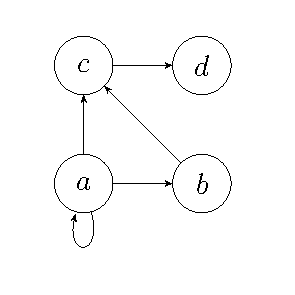
\includegraphics{graph.pdf}
\caption{Ориентированный граф.}
\label{fig1}
\end{figure}

\begin{figure}
\centering
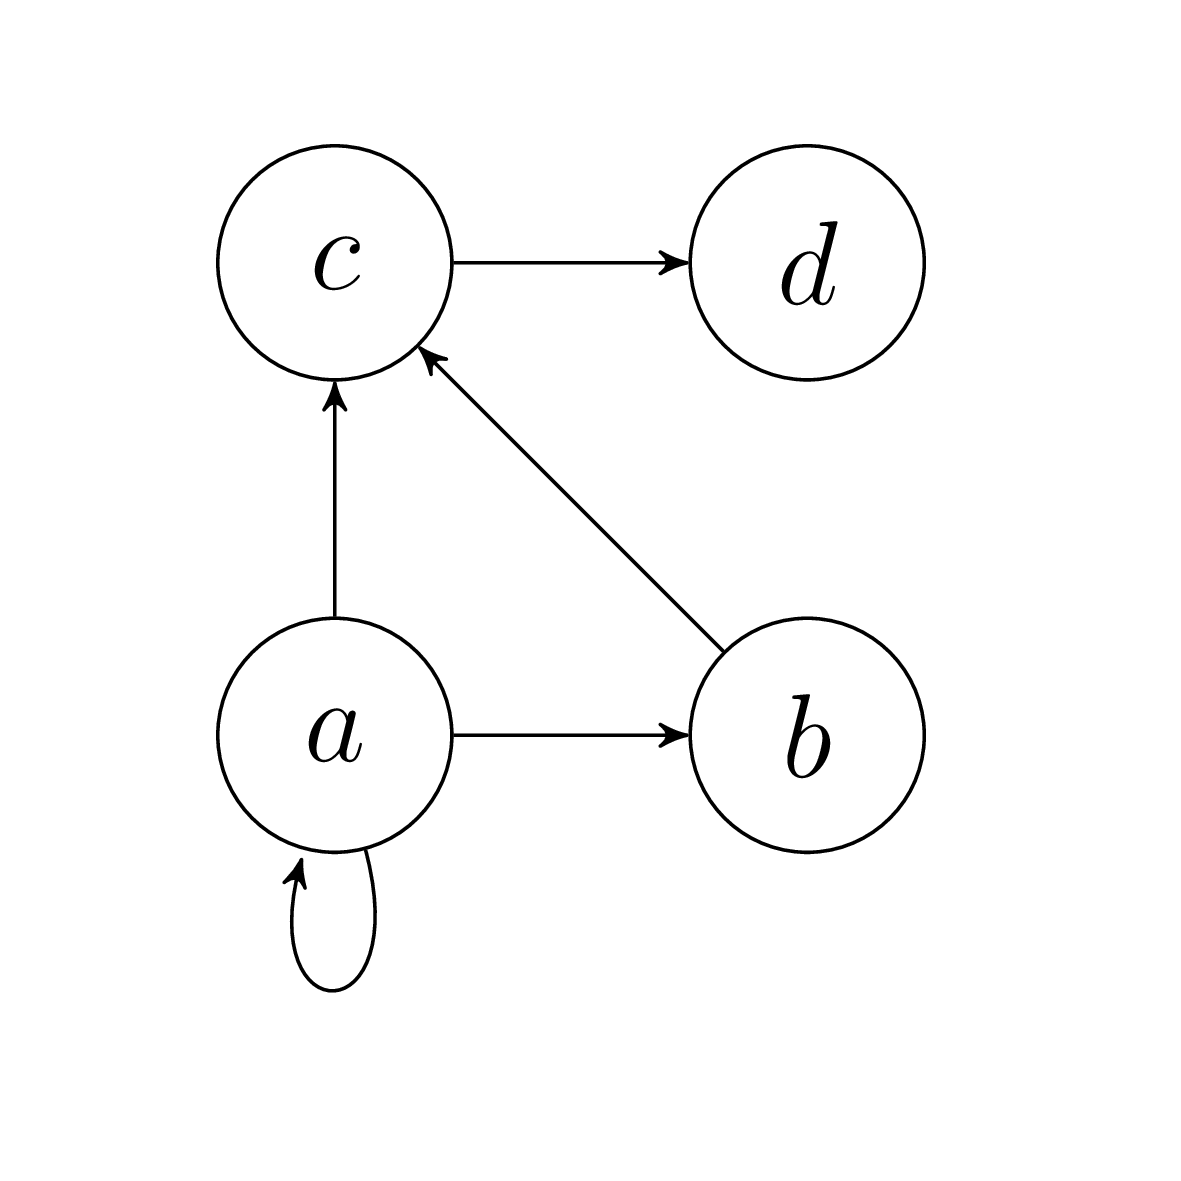
\includegraphics[width=0.5\textwidth]{graph.png}
\caption{Ориентированный граф.}
\label{fig2}
\end{figure}

\begin{figure}
\centering
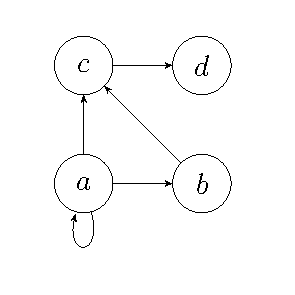
\includegraphics[scale=1.5]{graph.pdf}
\caption{Ориентированный граф.}
\label{fig3}
\end{figure}


\section{Определения и утверждения}

\begin{definition}
Множество $A$ называется подмножеством множества $B$, если любой элемент
множества $A$ принадлежит множеству~$B$.
\end{definition}

\begin{lemma}
Сумма двух нечетных чисел четна.
\end{lemma}
\begin{proof}
Очевидно.
\end{proof}

\begin{theorem}
\label{th1}
Любая циклическая группа является абелевой.
\end{theorem}
\begin{proof}[Схема доказательства]
См. любой учебник по алгебре.
\end{proof}

\begin{corollary}
Группа $(\mathbb Z,+)$ абелева.
\end{corollary}
\begin{proof}
Результат следует из теоремы~\ref{th1}.
\end{proof}

\begin{theorem}[Формула Байеса]
Для любых событий $A$ и $B$ таких, что $P(B) \neq 0$, справедливо равенство
$$P(A \mid B)=\frac{P(B \mid A)P(A)}{P(B)}.$$
\end{theorem}


\section{Библиография}

Список литературы должен содержать ссылки на основные книги и статьи,
использованные при написании диссертации. Ссылки упорядочиваются следующим
образом: сначала русские по алфавиту, потом английские по алфавиту.
Примеры ссылок: \cite{bib1}, \cite{bib2,bib4}, \cite{bib3,bib4,bib5},
\cite{bib6,bib7,bib8,bib9,bib11,bib12}, \cite[с.\,125]{bib10}.

\conclusion

Заключение содержит краткое подведение итогов проделанной работы
и возможные направления дальнейших исследований.

\begin{thebibliography}{99}
\bibitem{bib1}
Гонсалес, Р. Цифровая обработка изображений~/ Р.\,Гонсалес, Р.\,Вудс~;
пер. с англ. Л.\,И.\,Рубанова, П.\,А.\,Чочиа.~--- 3-е изд., испр. и
доп.~--- М.~: Техносфера, 2012.~--- 1104\,с.~--- URL: \url{https://www.technosphera.ru/files/book_pdf/0/book_311_455.pdf}

\bibitem{bib2}
Катаргин, Н.\,В. Оптимизация сетевого графика выполнения комплекса работ~//
Управленческие науки.~--- 2012.~--- №\,1.~--- С.\,87--93.~--- URL: \url{https://www.elibrary.ru/item.asp?id=18978098}

\bibitem{bib3}
Модели и методы теории логистики~: учебное пособие~/ В.\,С.\,Лукинский,
В.\,В.\,Лукинский, Ю.\,В.\,Малевич [и~др.]~--- 2-е изд.~--- СПб.~: Питер,
2007.~--- 448\,с.~--- URL: \url{https://www.elibrary.ru/item.asp?id=23948184}

\bibitem{bib4}
Орехов, Б. Атрибуция текста: теория и практика~: [сайт].~--- 2019.~---
6 июня.~--- URL: \url{https://postnauka.ru/faq/99046} (дата обращения:
08.05.2022).~--- Загл. с титул. экрана.

\bibitem{bib5}
Паттерны объектно-ориентированного проектирования~/ Э.\,Гамма, Р.\,Хелм,
Р.\,Джонсон, Д.\,Влиссидес~; пер. с англ. А.\,А.\,Слинкина.~--- СПб.~:
Питер, 2020.~--- 448\,с.~--- URL: \href{https://books.google.ru/books/about/\%D0\%9F\%D0\%B0\%D1\%82\%D1\%82\%D0\%B5\%D1\%80\%D0\%BD\%D1\%8B_\%D0\%BE\%D0\%B1\%D1\%8A\%D0\%B5\%D0\%BA\%D1\%82\%D0\%BD\%D0\%BE_\%D0\%BE\%D1\%80\%D0\%B8.html?hl=ru&id=1ZnsDwAAQBAJ&redir_esc=y}{\texttt{https://books.google.ru/books/about/Паттерны\_объектно\_\linebreak ори.html?hl=ru\&id=1ZnsDwAAQBAJ\&redir\_esc=y}}

\bibitem{bib6}
Feng, Y. The variance and covariance of fuzzy random variables and their
applications~/ Y.\,Feng, L.\,Hu, H.\,Shu~// Fuzzy Sets and Systems.~---
2001.~--- Vol.\,120, №\,2.~--- P.\,487--497.~--- DOI: \url{https://doi.org/10.1016/S0165-0114(99)00060-3}

\bibitem{bib7}
Goodfellow, I. Deep Learning~/ I.\,Goodfellow, Y.\,Bengio, A.\,Courvill.~--- Cambridge~: The MIT Press, 2016.~--- 800\,p.~--- URL: \url{https://www.deeplearningbook.org/}

\bibitem{bib8}
Harvey, A.\,C. Forecasting, Structural Time Series Models and the Kalman
Filter.~--- London~: Cambridge University Press, 1990.~--- 574\,p.~--- DOI: \url{https://doi.org/10.1017/CBO9781107049994}

\bibitem{bib9}
LSTM~// PyTorch~: [сайт].~--- URL:
\url{https://pytorch.org/docs/stable/generated/torch.nn.LSTM.html}
(дата обращения: 05.05.2022).~--- Загл. с титул. экрана.

\bibitem{bib10}
Nearest Neighbor Estimates of Entropy~/ H.\,Singh, V.\,Hnizdo, A.\,Demchuk
[et~al.]~// American Journal of Mathematical and Management Sciences.~---
2003.~--- Vol.\,23, №\,3.~--- P.\,301--321.~--- DOI: \url{https://doi.org/10.1080/01966324.2003.10737616}

\bibitem{bib11} Parallel Matrix Factorization for Recommender Systems~/
Y.\,Hsiang-Fu, C.-J.\,Hsien, S.\,Si, I.\,S.\,Dhillon~ // Knowledge and
Information Systems (KAIS).~--- 2014.~--- Vol.\,41, №\,3.~--- P.\,793--819.~--- DOI: \url{https://doi.org/10.1007/s10115-013-0682-2}

\bibitem{bib12}
\c{S}ent\"{u}rk, \.{I}. Factors Affecting the Notebook Computer Prices in
Turkey: A Hedonic Analysis~/ \.{I}.\,\c{S}ent\"{u}rk, C.\,Erdem~//
The Empirical Economics Letters.~--- 2010.~--- Vol.\,9, №\,6.~---
P.\,545--553.~--- URL: \url{https://www.researchgate.net/publication/261810646_Factors_Affecting_the_Notebook_Computer_Prices_in_Turkey_A_Hedonic_Analysis}
\end{thebibliography}

\end{paper}
\end{document}